\documentclass[aspectratio=169,11pt]{beamer}

% =========================================================
% PACKAGES
% =========================================================
\usepackage[utf8]{inputenc}
\usepackage[T1]{fontenc}
\usepackage{lmodern}
\usepackage{amsmath,amssymb}
\usepackage{booktabs}
\usepackage{array}
\usepackage{tikz}
\usepackage{ragged2e}
\usepackage{graphicx}
\usepackage[table]{xcolor}
\usepackage{hyperref}

\usetikzlibrary{
    arrows.meta,
    positioning,
    shapes.geometric,
    shapes.misc,
    fit,
    calc
}

% =========================================================
% COLORS
% =========================================================
\definecolor{AmritaMaroon}{RGB}{165,0,55}
\definecolor{AmritaDark}{RGB}{95,0,35}
\definecolor{LightBlue}{RGB}{220,237,250}
\definecolor{LightGreen}{RGB}{224,244,228}
\definecolor{LightOrange}{RGB}{252,235,205}
\definecolor{LightPink}{RGB}{250,225,235}
\definecolor{LightGray}{RGB}{242,242,242}

% =========================================================
% THEME
% =========================================================
\usetheme{default}

\setbeamertemplate{navigation symbols}{}

\setbeamertemplate{frametitle}{
    \vspace{0.15cm}
    \begin{beamercolorbox}[
        wd=\paperwidth,
        ht=0.85cm,
        dp=0.15cm,
        leftskip=0.35cm
    ]{frametitle}
        \color{white}
        \Large\insertframetitle
    \end{beamercolorbox}
}

\setbeamercolor{frametitle}{bg=AmritaMaroon}
\setbeamercolor{normal text}{fg=black}
\setbeamercolor{structure}{fg=AmritaMaroon}

% =========================================================
% CUSTOM COMMANDS
% =========================================================

\newcommand{\subtitleline}[1]{
    \vspace{-0.05cm}
    {\small\color{AmritaDark}\textit{#1}}
    \vspace{0.15cm}
}

\newcommand{\highlight}[1]{
    \textbf{\color{AmritaMaroon}#1}
}

\newcommand{\bulletitem}[2]{
    \item \textbf{#1} #2
}

\newcommand{\infobox}[4]{
    \begin{tikzpicture}
        \node[
            rounded corners=5pt,
            fill=#1,
            inner sep=9pt,
            text width=#2
        ] {
            \textbf{\color{AmritaMaroon}#3}\\[3pt]
            #4
        };
    \end{tikzpicture}
}

% =========================================================
% TITLE
% =========================================================

\title{
    \textbf{Smart Home HAR for}\\
    \textbf{Speech-Impaired \& Hearing-Impaired Users}
}

\author{
    23CSE399 -- Project Phase 2\\[3mm]
    \small
    Adhikkesh S K \quad
    Adithya Ajay \quad
    Amrith B\\
    Gowreesh B \quad
    Rishiikesh S K
}

\institute{
    Department of Computer Science and Engineering\\
    Amrita Vishwa Vidyapeetham
}

\date{
    Guide Review 1 \;|\; Panel Review 1
}

% =========================================================
% DOCUMENT
% =========================================================

\begin{document}

% =========================================================
% TITLE SLIDE
% =========================================================

\begin{frame}
    \begin{tikzpicture}[remember picture,overlay]

        % Top label
        \node[
            anchor=north east,
            fill=AmritaMaroon,
            text=white,
            rounded corners=3pt,
            inner xsep=10pt,
            inner ysep=5pt
        ] at ([xshift=-0.25cm,yshift=-0.2cm]current page.north east)
        {\scriptsize Type 2: Application Project};

    \end{tikzpicture}

    \vspace{0.7cm}

    \begin{center}
        {\color{AmritaMaroon}\Large\bfseries
        Smart Home HAR for}\\[0.15cm]

        {\color{AmritaMaroon}\LARGE\bfseries
        Speech-Impaired \& Hearing-Impaired Users}

        \vspace{0.45cm}

        {\large 23CSE399 -- Project Phase 2}\\
        {\large Guide Review 1 \;|\; Panel Review 1}

        \vspace{0.45cm}

        \begin{tabular}{c}
        Adhikkesh S K\\
        Adithya Ajay\\
        Amrith B\\
        Gowreesh B\\
        Rishiikesh S K
        \end{tabular}

        \vspace{0.35cm}

        \textbf{Guide: Ms. Nalinadevi K}\\
        Department of CSE, Amrita Vishwa Vidyapeetham
    \end{center}
\end{frame}


% =========================================================
% 1. USE CASES
% =========================================================

\begin{frame}{1. Motivation}

\begin{itemize}
    \setlength{\itemsep}{0.45em}
    \setlength{\parskip}{0pt}

    \item \textcolor{blue}{\textbf{Smart Homes:}}
    Rapid adoption --- \textbf{82.1\% projected increase in smarthome systems by 2026}
    \hspace{0.2em}\textit{\small (Statista)}

    \item \textcolor{blue}{\textbf{Accessibility:}}
    \textbf{1.5 billion} people with hearing loss
    $\rightarrow$ \textbf{2.5 billion by 2050}
    \hspace{0.1em}\textit{\small (WHO)}

    \item \textcolor{blue}{\textbf{Sign-Language Recognition:}}
    Since \textbf{1991} --- predominantly
    \textbf{camera/image- or wearable sensor-based recognition}

    \item \textcolor{blue}{\textbf{Human Activity Recognition:}}
    Predominantly \textbf{single-modality sensing}
    $\rightarrow$ limited information from one sensing source

    \item \textcolor{blue}{\textbf{Privacy:}}
    \textbf{87\% of reviewed studies} reported privacy concerns
    with smart-home surveillance
    \hspace{0.2em}\textit{\small (JMIR Scoping Review)}

\end{itemize}

\vspace{0.2cm}

\begin{beamercolorbox}[
    rounded=true,
    sep=0.6em,
    wd=\textwidth
]{block body}

\small
Most existing systems rely on \textbf{single-modality sensing},
limiting recognition of \textbf{activities, sign language, interactions,
and intent}. Along with \textbf{camera privacy concerns} and the need
for \textbf{accessible smart homes}, this motivates a
\textbf{multimodal, privacy-preserving approach}.

\end{beamercolorbox}

\end{frame}


% =========================================================
% 2. USE CASE 3
% =========================================================

\begin{frame}{2. Introduction}

\begin{itemize}
    \setlength{\itemsep}{0.5em}

    \item \textcolor{blue}{\textbf{Context Awareness:}}
    \textit{What is happening?}
    $\rightarrow$ Person sitting, walking, cooking

    \item \textcolor{blue}{\textbf{Intent Awareness:}}
    \textit{Why is it happening?}
    $\rightarrow$ Sitting to rest, walking to leave, reaching to switch off a light

    \item \textcolor{blue}{\textbf{Context $\neq$ Intent:}}
    The same activity can represent \textbf{different intentions}
    depending on the situation.

    \item \textcolor{blue}{\textbf{Real-World Complexity:}}
    \textbf{Multiple people + simultaneous activities + interactions}
    make intent harder to infer.

    \item \textcolor{blue}{\textbf{Beyond Activity Recognition:}}
    Understanding \textbf{who is doing what, with whom, and why}
    enables more meaningful automation.

    \item \textcolor{blue}{\textbf{Our Goal:}}
    Move from \textbf{activity recognition}
    $\rightarrow$ \textbf{context understanding}
    $\rightarrow$ \textbf{intent-aware smart-home decisions}.
\end{itemize}

\end{frame}


% =========================================================
% 3. MOTIVATION
% =========================================================

\begin{frame}{3. Motivation: Why Move to a Controlled SDR-Based CSI System?}

\vspace{0.15cm}

\begin{columns}[T,totalwidth=\textwidth]

% ---------------------------------------------------------
% LEFT COLUMN
% ---------------------------------------------------------

\column{0.48\textwidth}

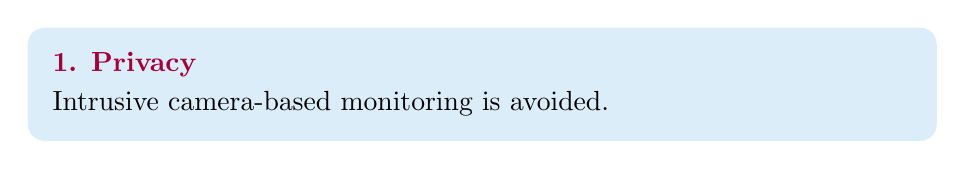
\begin{tikzpicture}
\node[
    rounded corners=6pt,
    fill=LightBlue,
    inner sep=9pt,
    text width=0.90\textwidth,
    align=left
] {
    \textbf{\color{AmritaMaroon}1. Privacy}\\[2pt]
    Intrusive camera-based monitoring is avoided.
};
\end{tikzpicture}

\vspace{0.16cm}

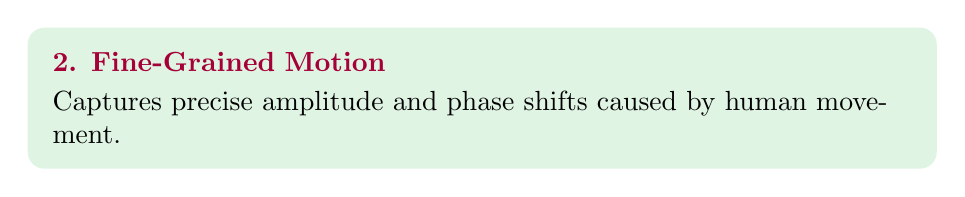
\begin{tikzpicture}
\node[
    rounded corners=6pt,
    fill=LightGreen,
    inner sep=9pt,
    text width=0.90\textwidth,
    align=left
] {
    \textbf{\color{AmritaMaroon}2. Fine-Grained Motion}\\[2pt]
    Captures precise amplitude and phase shifts caused by human movement.
};
\end{tikzpicture}

\vspace{0.16cm}

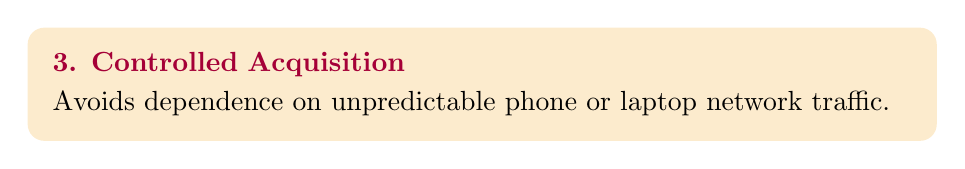
\begin{tikzpicture}
\node[
    rounded corners=6pt,
    fill=LightOrange,
    inner sep=9pt,
    text width=0.90\textwidth,
    align=left
] {
    \textbf{\color{AmritaMaroon}3. Controlled Acquisition}\\[2pt]
    Avoids dependence on unpredictable phone or laptop network traffic.
};
\end{tikzpicture}


% ---------------------------------------------------------
% RIGHT COLUMN
% ---------------------------------------------------------

\column{0.48\textwidth}

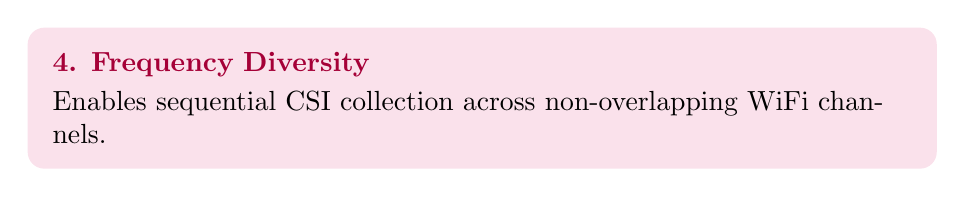
\begin{tikzpicture}
\node[
    rounded corners=6pt,
    fill=LightPink,
    inner sep=9pt,
    text width=0.90\textwidth,
    align=left
] {
    \textbf{\color{AmritaMaroon}4. Frequency Diversity}\\[2pt]
    Enables sequential CSI collection across non-overlapping WiFi channels.
};
\end{tikzpicture}

\vspace{0.16cm}

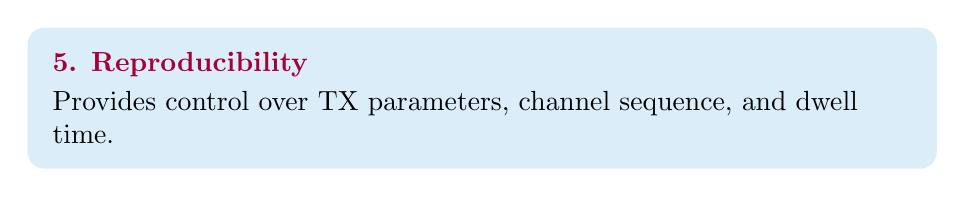
\begin{tikzpicture}
\node[
    rounded corners=6pt,
    fill=LightBlue,
    inner sep=9pt,
    text width=0.90\textwidth,
    align=left
] {
    \textbf{\color{AmritaMaroon}5. Reproducibility}\\[2pt]
    Provides control over TX parameters, channel sequence, and dwell time.
};
\end{tikzpicture}

\vspace{0.35cm}

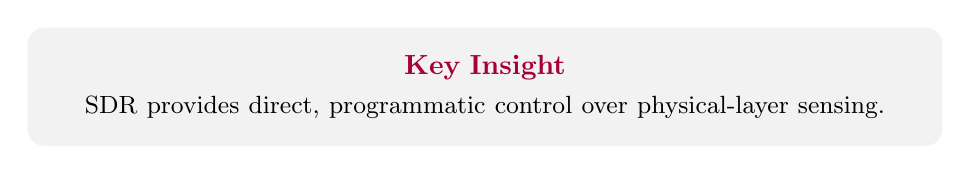
\begin{tikzpicture}
\node[
    rounded corners=6pt,
    fill=LightGray,
    inner sep=10pt,
    text width=0.90\textwidth,
    align=center
] {
    \textbf{\color{AmritaMaroon}Key Insight}\\[2pt]
    \small
    SDR provides direct, programmatic control over
    physical-layer sensing.
};
\end{tikzpicture}

\end{columns}

\end{frame}


% =========================================================
% 4. PROBLEM STATEMENT
% =========================================================

\begin{frame}{4. Problem Statement \& Research Objectives}
\subtitleline{Building a controlled, privacy-preserving CSI-HAR pipeline}

\vspace{-0.2cm}

\begin{center}
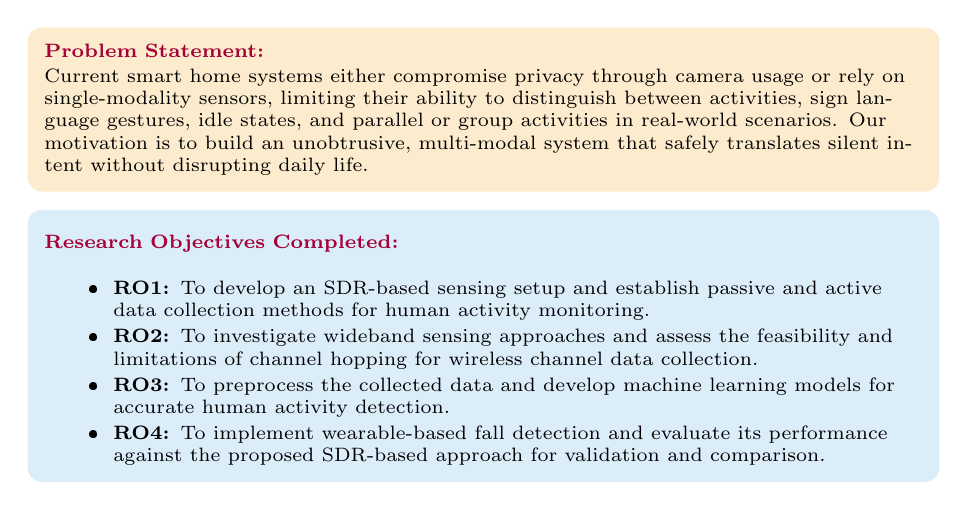
\begin{tikzpicture}

% ---------------------------------------------------------
% PROBLEM STATEMENT
% ---------------------------------------------------------
\node[
    rounded corners=5pt,
    fill=LightOrange,
    inner sep=6pt,
    text width=0.92\textwidth,
    align=left,
    font=\scriptsize
] (prob) {
\textbf{\color{AmritaMaroon}Problem Statement:}\\[1pt]
Current smart home systems either compromise privacy through camera usage or rely on
single-modality sensors, limiting their ability to distinguish between activities, sign
language gestures, idle states, and parallel or group activities in real-world scenarios.
Our motivation is to build an unobtrusive, multi-modal system that safely translates
silent intent without disrupting daily life.
};

% ---------------------------------------------------------
% RESEARCH OBJECTIVES
% ---------------------------------------------------------
\node[
    rounded corners=5pt,
    fill=LightBlue,
    below=0.22cm of prob,
    inner sep=6pt,
    text width=0.92\textwidth,
    align=left,
    font=\scriptsize
] (obj) {

\textbf{\color{AmritaMaroon}Research Objectives Completed:}

\vspace{-0.05cm}

\begin{itemize}
    \setlength\itemsep{0.18em}
    \setlength\parskip{0pt}
    \setlength\parsep{0pt}
    \setlength{\leftskip}{0pt}

    \item \textbf{RO1:} To develop an SDR-based sensing setup and establish passive and active
    data collection methods for human activity monitoring.

    \item \textbf{RO2:} To investigate wideband sensing approaches and assess the feasibility
    and limitations of channel hopping for wireless channel data collection.

    \item \textbf{RO3:} To preprocess the collected data and develop machine learning models
    for accurate human activity detection.

    \item \textbf{RO4:} To implement wearable-based fall detection and evaluate its
    performance against the proposed SDR-based approach for validation and comparison.

\end{itemize}
};

\end{tikzpicture}
\end{center}

\end{frame}

% =========================================================
% 4b. OBJECTIVES TO BE COMPLETED
% =========================================================

\begin{frame}{4.  Problem Statement \& Research Objectives}

\vspace{-0.1cm}
\begin{center}
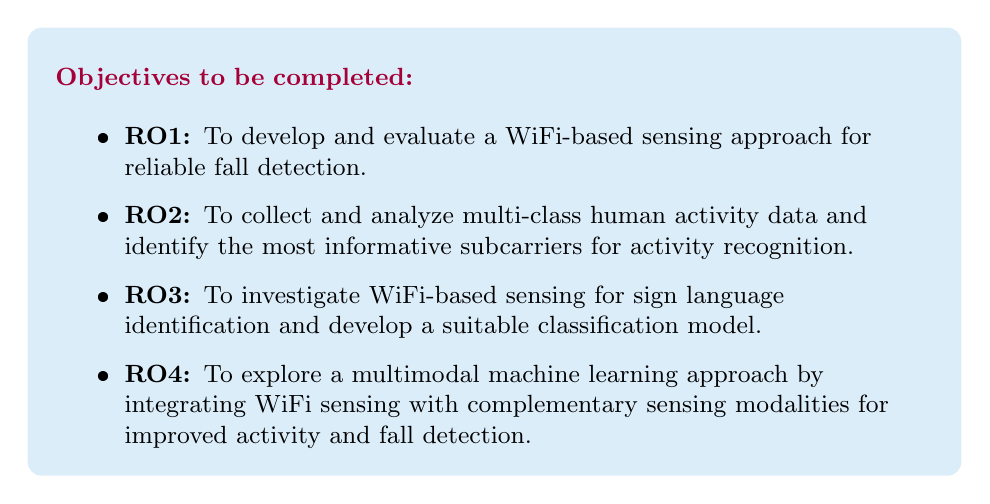
\begin{tikzpicture}[node distance=0.3cm]

\node[
    rounded corners=5pt,
    fill=LightBlue,
    inner sep=10pt,
    text width=0.92\textwidth,
    align=left,
    font=\small
] (future_obj) {

\textbf{\color{AmritaMaroon}Objectives to be completed:}

\vspace{0.15cm}
\begin{itemize}
    \setlength\itemsep{0.5em}
    \item \textbf{RO1:} To develop and evaluate a WiFi-based sensing approach for reliable fall detection.
    
    \item \textbf{RO2:} To collect and analyze multi-class human activity data and identify the most informative subcarriers for activity recognition.
    
    \item \textbf{RO3:} To investigate WiFi-based sensing for sign language identification and develop a suitable classification model.
    
    \item \textbf{RO4:} To explore a multimodal machine learning approach by integrating WiFi sensing with complementary sensing modalities for improved activity and fall detection.
\end{itemize}
};

\end{tikzpicture}
\end{center}

\end{frame}
% =========================================================
% 5. LITERATURE SURVEY
% =========================================================

\begin{frame}{5. Literature Survey}

\vspace{0.1cm}
\centering
\scriptsize
\renewcommand{\arraystretch}{1.25}
\setlength{\tabcolsep}{4pt}
\begin{tabular}{>{\bfseries\RaggedRight\arraybackslash}p{0.20\textwidth} >{\RaggedRight\arraybackslash}p{0.32\textwidth} >{\RaggedRight\arraybackslash}p{0.40\textwidth}}
\toprule
\rowcolor{AmritaMaroon}
{\color{white}Paper (Year)} & {\color{white}\textbf{Method / Technique}} & {\color{white}\textbf{Description}} \\
\midrule

\rowcolor{LightBlue}
SignFi \par (2018) &
9-layer CNN on WiFi CSI amplitude and phase &
Recognizes 276 sign-language gestures with 98\% lab accuracy; accuracy falls to 67\% for users unseen during training. \\
\midrule

\rowcolor{LightGreen}
Widar3.0 \par (2021) &
Domain-independent Body-coordinate Velocity Profile (BVP) + CNN--GRU &
Achieves zero-effort cross-domain gesture recognition (83--92\%), but requires line-of-sight and multiple synchronized WiFi links. \\
\midrule

\rowcolor{LightOrange}
ImgFi \par (2023) &
CSI converted to Recurrence-Plot images, classified by a lightweight 2D-CNN &
Reaches 99.5--99.8\% accuracy with $\sim$90$\times$ fewer parameters than ResNet50, but is evaluated within-domain only. \\
\midrule

\rowcolor{LightPink}
Joint Activity \& Localization \par (2019) &
Dual-branch 1D-CNN (ResNet1D) on CSI subcarrier fingerprints &
Jointly predicts activity (88\%) and indoor location (95.7\%) from CSI, but on a single-user, single-room dataset. \\
\bottomrule
\end{tabular}

\vspace{6pt}
\raggedright
{\color{AmritaMaroon}\scriptsize\bfseries Takeaway: }{\scriptsize Existing WiFi CSI systems are single-purpose (gesture-only or localization-only) and environment-specific. Our controlled multi-channel CSI pipeline aims to unify activity and sign-transition recognition in one privacy-preserving system.\par}

\end{frame}


% =========================================================
% 6. SYSTEM EVOLUTION + CURRENT ARCHITECTURE
% =========================================================

\begin{frame}{6. System Evolution: From Passive Capture to Controlled CSI}
\subtitleline{The major implementation change in the current phase}

\vspace{0.15cm}

\begin{columns}[T,totalwidth=\textwidth]

% ---------------- PREVIOUS ----------------

\column{0.45\textwidth}

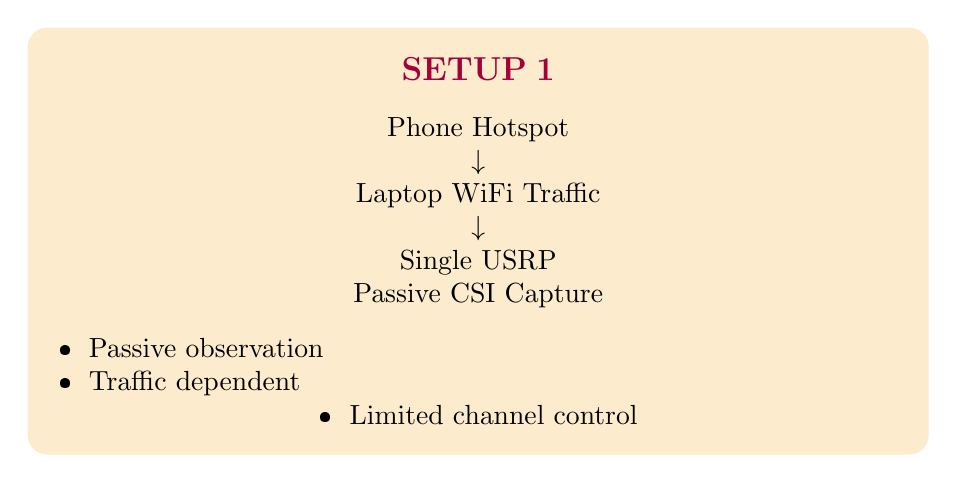
\begin{tikzpicture}
\node[
    rounded corners=7pt,
    fill=LightOrange,
    inner sep=11pt,
    text width=0.88\textwidth,
    align=center
] {
    {\large\bfseries\color{AmritaMaroon} SETUP 1}\\[8pt]

    Phone Hotspot\\
    $\downarrow$\\
    Laptop WiFi Traffic\\
    $\downarrow$\\
    Single USRP\\
    Passive CSI Capture\\[8pt]

    \raggedright
    \textbullet\; Passive observation\\
    \textbullet\; Traffic dependent\\
    \textbullet\; Limited channel control
};
\end{tikzpicture}

% ---------------- ARROW ----------------

\column{0.08\textwidth}

\begin{center}
\vspace{1.8cm}
{\Huge $\Rightarrow$}
\end{center}

% ---------------- CURRENT ----------------

\column{0.45\textwidth}

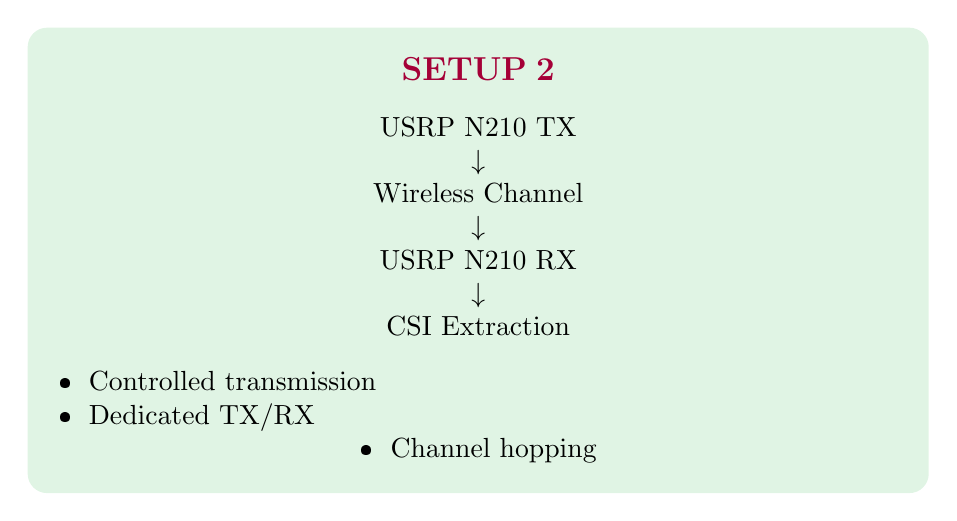
\begin{tikzpicture}
\node[
    rounded corners=7pt,
    fill=LightGreen,
    inner sep=11pt,
    text width=0.88\textwidth,
    align=center
] {
    {\large\bfseries\color{AmritaMaroon}SETUP 2}\\[8pt]

    USRP N210 TX\\
    $\downarrow$\\
    Wireless Channel\\
    $\downarrow$\\
    USRP N210 RX\\
    $\downarrow$\\
    CSI Extraction\\[8pt]

    \raggedright
    \textbullet\; Controlled transmission\\
    \textbullet\; Dedicated TX/RX\\
    \textbullet\; Channel hopping
};
\end{tikzpicture}

\end{columns}

\vspace{0.35cm}

\begin{center}
\textbf{\color{AmritaMaroon}Key change:}
From passive WiFi observation to a controlled SDR-based CSI platform.
\end{center}

\end{frame}


% =========================================================
% 7. CURRENT IMPLEMENTATION
% =========================================================

\begin{frame}{7. Current Implementation: Two-USRP CSI Setup}
\subtitleline{Controlled IEEE 802.11 transmission and sequential channel hopping}

\vspace{0.3cm}

\begin{center}

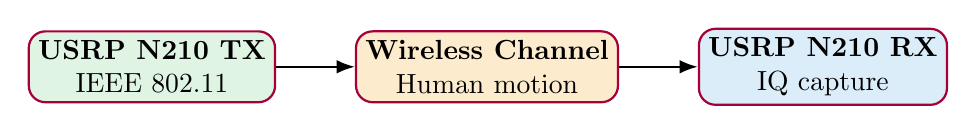
\begin{tikzpicture}[
    box/.style={
        rounded corners=6pt,
        minimum width=3.0cm,
        minimum height=0.9cm,
        align=center,
        draw=AmritaMaroon,
        thick
    },
    arr/.style={-{Latex},thick}
]

\node[box,fill=LightGreen] (tx)
{\textbf{USRP N210 TX}\\IEEE 802.11};

\node[box,fill=LightOrange,right=1.0cm of tx] (air)
{\textbf{Wireless Channel}\\Human motion};

\node[box,fill=LightBlue,right=1.0cm of air] (rx)
{\textbf{USRP N210 RX}\\IQ capture};

\draw[arr] (tx)--(air);
\draw[arr] (air)--(rx);

\end{tikzpicture}

\vspace{0.65cm}

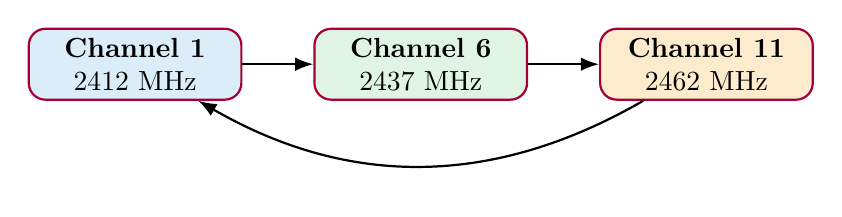
\begin{tikzpicture}[
    ch/.style={
        rounded corners=6pt,
        minimum width=2.7cm,
        minimum height=0.78cm,
        align=center,
        draw=AmritaMaroon,
        thick
    },
    arr/.style={-{Latex},thick}
]

\node[ch,fill=LightBlue] (c1)
{\textbf{Channel 1}\\2412 MHz};

\node[ch,fill=LightGreen,right=0.9cm of c1] (c6)
{\textbf{Channel 6}\\2437 MHz};

\node[ch,fill=LightOrange,right=0.9cm of c6] (c11)
{\textbf{Channel 11}\\2462 MHz};

\draw[arr] (c1)--(c6);
\draw[arr] (c6)--(c11);
\draw[arr] (c11) to[bend left=30] (c1);

\end{tikzpicture}

\vspace{0.5cm}

\begin{columns}[T,totalwidth=\textwidth]

\column{0.48\textwidth}

\begin{itemize}
    \item Controlled IEEE 802.11 transmission
    \item Dedicated SDR transmitter and receiver
\end{itemize}

\column{0.48\textwidth}

\begin{itemize}
    \item Sequential hopping across Channels 1, 6 and 11
    \item $\approx$100 ms dwell per channel
\end{itemize}

\end{columns}

\end{center}

\end{frame}

% =========================================================
% 8. CSI TRANSMISSION PIPELINE
% =========================================================

\begin{frame}{8. CSI Transmission Pipeline}
\subtitleline{Transmitting 802.11 frames to extract CSI}

\begin{center}

\includegraphics[
    width=0.9\textwidth,
    height=4.5cm,
    keepaspectratio
]{tx_gnuradio.png}

\vspace{0.15cm}

\textbf{\color{AmritaMaroon}Key result:}

Network payloads are encoded into 802.11 WiFi frames and
transmitted via USRP to enable continuous channel measurement.

\end{center}

\end{frame}

% =========================================================
% 9. CSI ACQUISITION PIPELINE
% =========================================================

\begin{frame}{8. CSI Acquisition Pipeline}
\subtitleline{Processing received 802.11 frames to extract CSI}


\begin{center}

% Replace 'your_image_filename.png' with your actual image file name
\includegraphics[width=0.85\textwidth, keepaspectratio]{rx_gnuradio.png}

\vspace{0.2cm}

\textbf{\color{AmritaMaroon}Key result:}
Received WiFi frames are converted into CSI measurements
for subsequent HAR analysis.

\end{center}

\end{frame}
% =========================================================
% 9. MODEL ARCHITECTURE & METHODOLOGY
% =========================================================

\begin{frame}{9. Model Architecture \& Methodology}
\subtitleline{CSI-based activity classification using Recurrence Plots and ResNet-18}

\vspace{0.2cm}

\begin{columns}[T,onlytextwidth]

\column{0.62\textwidth}

\begin{center}

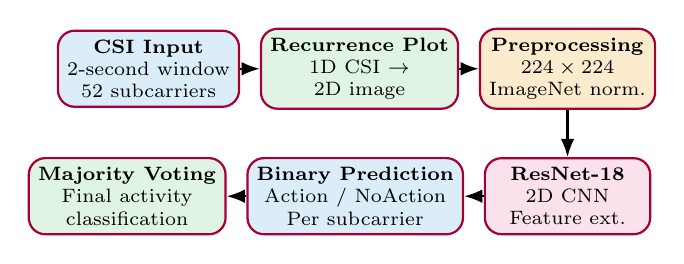
\begin{tikzpicture}[
    box/.style={
        rounded corners=6pt,
        minimum width=2.1cm,
        minimum height=0.9cm,
        align=center,
        draw=AmritaMaroon,
        thick,
        font=\scriptsize
    },
    arr/.style={-{Latex},thick}
]

% Top Row: Left to Right
\node[box,fill=LightBlue] (input)
{\textbf{CSI Input}\\
2-second window\\
52 subcarriers};

\node[box,fill=LightGreen,right=0.25cm of input] (rp)
{\textbf{Recurrence Plot}\\
1D CSI $\rightarrow$\\
2D image};

\node[box,fill=LightOrange,right=0.25cm of rp] (prep)
{\textbf{Preprocessing}\\
$224\times224$\\
ImageNet norm.};

% Bottom Row: Right to Left (Forms a clean U-Shape flow)
\node[box,fill=LightPink,below=0.6cm of prep] (resnet)
{\textbf{ResNet-18}\\
2D CNN\\
Feature ext.};

\node[box,fill=LightBlue,left=0.25cm of resnet] (prediction)
{\textbf{Binary Prediction}\\
Action / NoAction\\
Per subcarrier};

\node[box,fill=LightGreen,left=0.25cm of prediction] (voting)
{\textbf{Majority Voting}\\
Final activity\\
classification};

% Arrows mapping the U-Shape pipeline
\draw[arr] (input) -- (rp);
\draw[arr] (rp) -- (prep);
\draw[arr] (prep) -- (resnet);
\draw[arr] (resnet) -- (prediction);
\draw[arr] (prediction) -- (voting);

\end{tikzpicture}

\vspace{0.4cm}

\textbf{\color{AmritaMaroon}Training:}\\
Adam optimizer + dynamic learning-rate scheduling

\end{center}

\column{0.35\textwidth}

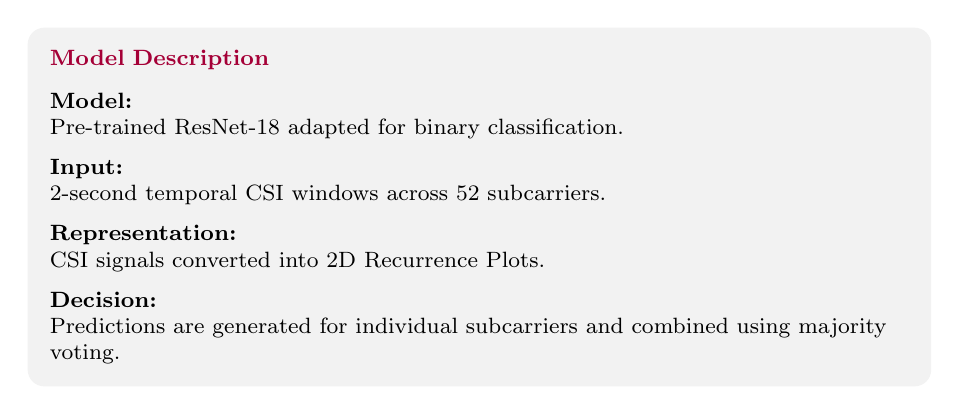
\begin{tikzpicture}
\node[
    rounded corners=6pt,
    fill=LightGray,
    inner sep=8pt,
    text width=0.9\linewidth, % Bound to column width
    align=left,
    font=\footnotesize
] {
\textbf{\color{AmritaMaroon}Model Description}\\[6pt]

\textbf{Model:}\\
Pre-trained ResNet-18 adapted for binary classification.\\[5pt]

\textbf{Input:}\\
2-second temporal CSI windows across 52 subcarriers.\\[5pt]

\textbf{Representation:}\\
CSI signals converted into 2D Recurrence Plots.\\[5pt]

\textbf{Decision:}\\
Predictions are generated for individual subcarriers and combined using majority voting.
};
\end{tikzpicture}

\end{columns}

\end{frame}


% =========================================================
% 10. MODEL RESULTS
% =========================================================

\begin{frame}{10. Model Performance \& Results}

\begin{columns}[T,onlytextwidth]

\column{0.48\textwidth}
\begin{center}

\textbf{\color{AmritaMaroon}Confusion Matrix}

\vspace{0.1cm}

\includegraphics[
    width=0.9\linewidth,
    height=3.3cm,
    keepaspectratio
]{plot.png}

\vspace{0.25cm}

\textbf{\color{AmritaMaroon}Classification Report}

\vspace{0.1cm}

\scriptsize
\renewcommand{\arraystretch}{1.2}
\begin{tabular}{lccc}
\toprule
\textbf{Class} & \textbf{Precision} & \textbf{Recall} & \textbf{F1} \\
\midrule
NoAction & 0.93 & 0.99 & 0.96 \\
Action   & 0.99 & 0.93 & 0.96 \\
\midrule
\textbf{Overall} & \textbf{0.96} & \textbf{0.96} & \textbf{0.96} \\
\bottomrule
\end{tabular}

\end{center}

\column{0.48\textwidth}
\begin{center}

\textbf{\color{AmritaMaroon}Training \& Validation Accuracy}

\vspace{0.1cm}

\includegraphics[
    width=0.9\linewidth,
    height=3.3cm,
    keepaspectratio
]{WhatsApp Image 2026-08-13 at 11.02.06 PM.jpeg}

\vspace{0.25cm}

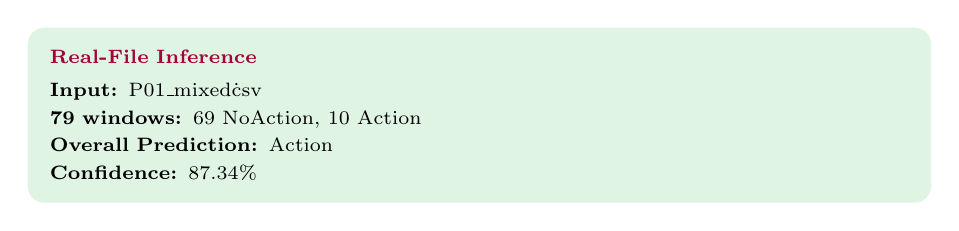
\begin{tikzpicture}
\node[
    rounded corners=6pt,
    fill=LightGreen,
    inner sep=8pt,
    text width=0.9\linewidth,
    align=left,
    font=\scriptsize
] {
\textbf{\color{AmritaMaroon}Real-File Inference}\\[4pt]
\textbf{Input:} P01\_mixed\.csv\\[2pt]
\textbf{79 windows:} 69 NoAction, 10 Action\\[2pt]
\textbf{Overall Prediction:} Action\\[2pt]
\textbf{Confidence:} 87.34\%
};
\end{tikzpicture}

\end{center}
\end{columns}

\vspace{0.3cm}

\begin{center}
\large\textbf{\color{AmritaMaroon}Overall Classification Accuracy: 96\%}
\end{center}

\end{frame}
% =========================================================
% 9. IMPORTANT DISTINCTION
% =========================================================

\begin{frame}{11. Current Capability vs. Future Extension}
\subtitleline{Clarifying what the present implementation achieves}

\begin{columns}[T]

% =========================================================
% CURRENT
% =========================================================

\column{0.47\textwidth}

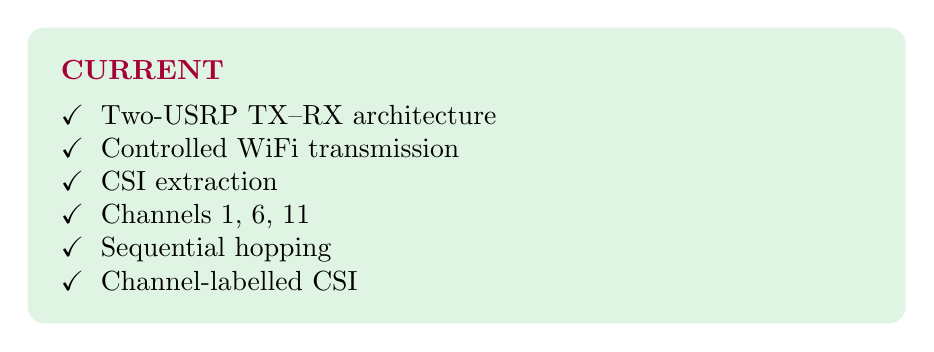
\begin{tikzpicture}
\node[
    rounded corners=6pt,
    fill=LightGreen,
    inner sep=12pt,
    text width=0.85\textwidth,
    align=left
] {
\textbf{\color{AmritaMaroon}CURRENT}\\[4pt]

\checkmark\; Two-USRP TX--RX architecture\\
\checkmark\; Controlled WiFi transmission\\
\checkmark\; CSI extraction\\
\checkmark\; Channels 1, 6, 11\\
\checkmark\; Sequential hopping\\
\checkmark\; Channel-labelled CSI
};
\end{tikzpicture}

% =========================================================
% FUTURE
% =========================================================

\column{0.47\textwidth}

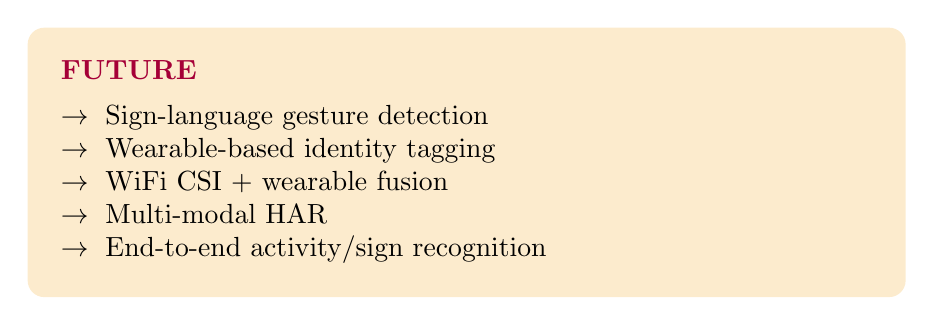
\begin{tikzpicture}
\node[
    rounded corners=6pt,
    fill=LightOrange,
    inner sep=12pt,
    text width=0.85\textwidth,
    align=left
] {
\textbf{\color{AmritaMaroon}FUTURE}\\[4pt]

$\rightarrow$\; Sign-language gesture detection\\
$\rightarrow$\; Wearable-based identity tagging\\
$\rightarrow$\; WiFi CSI + wearable fusion\\
$\rightarrow$\; Multi-modal HAR\\
$\rightarrow$\; End-to-end activity/sign recognition
};
\end{tikzpicture}

\end{columns}

\vspace{0.45cm}

\begin{center}
\textbf{Important:}
The present two-USRP system hops between channels; it does
\textbf{not} receive Channels 1, 6 and 11 simultaneously.
\end{center}

\end{frame}
% =========================================================
% 12. CSI DATA    [SPACING FIXED - was overflowing]
% =========================================================

\begin{frame}{12. CSI Data: From Channel Response to HAR Input}
\subtitleline{What is extracted from each received WiFi frame}

\begin{center}

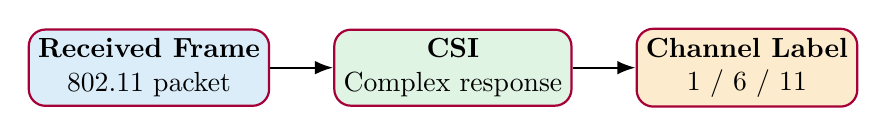
\begin{tikzpicture}[
    box/.style={
        rounded corners=6pt,
        minimum width=2.7cm,
        minimum height=0.78cm,
        align=center,
        draw=AmritaMaroon,
        thick
    },
    arr/.style={-{Latex},thick}
]

\node[box,fill=LightBlue] (frame)
{\textbf{Received Frame}\\802.11 packet};

\node[box,fill=LightGreen,right=0.8cm of frame] (csi)
{\textbf{CSI}\\Complex response};

\node[box,fill=LightOrange,right=0.8cm of csi] (label)
{\textbf{Channel Label}\\1 / 6 / 11};

\draw[arr] (frame)--(csi);
\draw[arr] (csi)--(label);

\end{tikzpicture}

\vspace{0.35cm}

\begin{columns}[T,totalwidth=\textwidth]

\column{0.48\textwidth}

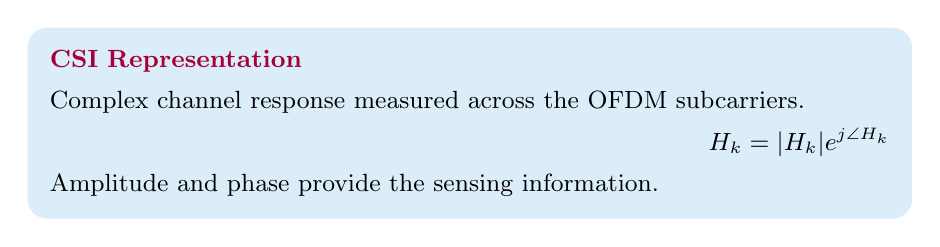
\begin{tikzpicture}
\node[
    rounded corners=7pt,
    fill=LightBlue,
    inner sep=8pt,
    text width=0.88\textwidth,
    align=left,
    font=\small
] {
\textbf{\color{AmritaMaroon}CSI Representation}\\[4pt]

Complex channel response measured across
the OFDM subcarriers.\\[4pt]

\hspace*{\fill}$H_k = |H_k|e^{j\angle H_k}$\hspace*{\fill}\\[4pt]

Amplitude and phase provide the sensing information.
};
\end{tikzpicture}

\column{0.48\textwidth}

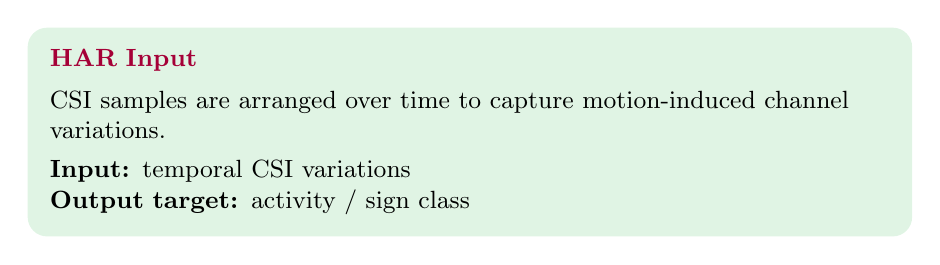
\begin{tikzpicture}
\node[
    rounded corners=7pt,
    fill=LightGreen,
    inner sep=8pt,
    text width=0.88\textwidth,
    align=left,
    font=\small
] {
\textbf{\color{AmritaMaroon}HAR Input}\\[4pt]

CSI samples are arranged over time to capture
motion-induced channel variations.

\vspace{3pt}

\textbf{Input:} temporal CSI variations\\
\textbf{Output target:} activity / sign class
};
\end{tikzpicture}

\end{columns}

\vspace{0.25cm}

{\small\textbf{\color{AmritaMaroon}Key result:}
Each CSI sample is associated with the active WiFi channel,
enabling channel-aware HAR analysis.}

\end{center}

\end{frame}

% =========================================================
% 11. CSI PROCESSING AND SOFTWARE ARCHITECTURE
% =========================================================

\begin{frame}{13. CSI Processing and Software Architecture}
\subtitleline{GNU Radio + UHD + Python channel control + custom CSI extraction}

\vspace{0.1cm}

\begin{center}

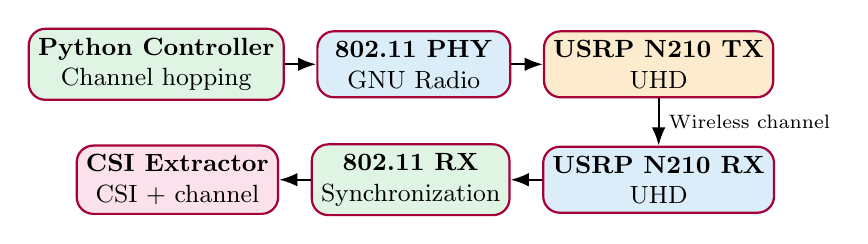
\begin{tikzpicture}[
    box/.style={
        rounded corners=6pt,
        minimum width=2.45cm,
        minimum height=0.6cm, % Reduced height slightly
        align=center,
        draw=AmritaMaroon,
        thick,
        font=\small % Added to reduce text size slightly
    },
    arr/.style={-{Latex},thick}
]

% =========================================================
% TX SIDE
% =========================================================

\node[
    box,
    fill=LightGreen
] (controller)
{\textbf{Python Controller}\\Channel hopping};

\node[
    box,
    fill=LightBlue,
    right=0.4cm of controller % Tightened gap
] (txphy)
{\textbf{802.11 PHY}\\GNU Radio};

\node[
    box,
    fill=LightOrange,
    right=0.4cm of txphy % Tightened gap
] (txusrp)
{\textbf{USRP N210 TX}\\UHD};

% =========================================================
% RX SIDE
% =========================================================

\node[
    box,
    fill=LightBlue,
    below=0.6cm of txusrp % Tightened vertical gap
] (rxusrp)
{\textbf{USRP N210 RX}\\UHD};

\node[
    box,
    fill=LightGreen,
    left=0.4cm of rxusrp % Tightened gap
] (sync)
{\textbf{802.11 RX}\\Synchronization};

\node[
    box,
    fill=LightPink,
    left=0.4cm of sync % Tightened gap
] (csi)
{\textbf{CSI Extractor}\\CSI + channel};

% =========================================================
% CONNECTIONS
% =========================================================

\draw[arr] (controller)--(txphy);
\draw[arr] (txphy)--(txusrp);

\draw[arr] (txusrp) -- node[right,font=\scriptsize]
{Wireless channel} (rxusrp);

\draw[arr] (rxusrp)--(sync);
\draw[arr] (sync)--(csi);

\end{tikzpicture}

\vspace{0.2cm} % Reduced vertical space

\begin{columns}[T,totalwidth=\textwidth]

\column{0.48\textwidth}

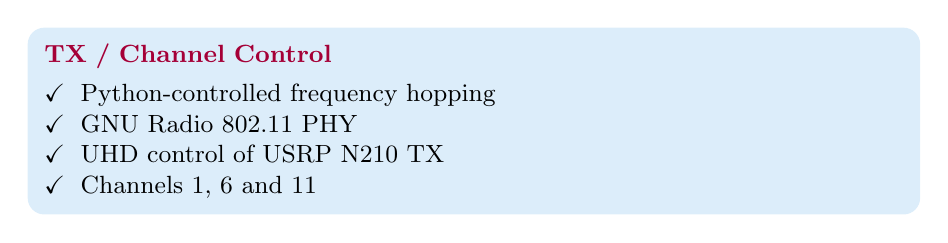
\begin{tikzpicture}
\node[
    rounded corners=6pt,
    fill=LightBlue,
    inner sep=6pt, % Reduced padding
    text width=0.9\textwidth,
    align=left,
    font=\small % Scaled down font to prevent word wrap overflow
] {
\textbf{\color{AmritaMaroon}TX / Channel Control}\\[3pt]
$\checkmark$\; Python-controlled frequency hopping\\
$\checkmark$\; GNU Radio 802.11 PHY\\
$\checkmark$\; UHD control of USRP N210 TX\\
$\checkmark$\; Channels 1, 6 and 11
};
\end{tikzpicture}

\column{0.48\textwidth}

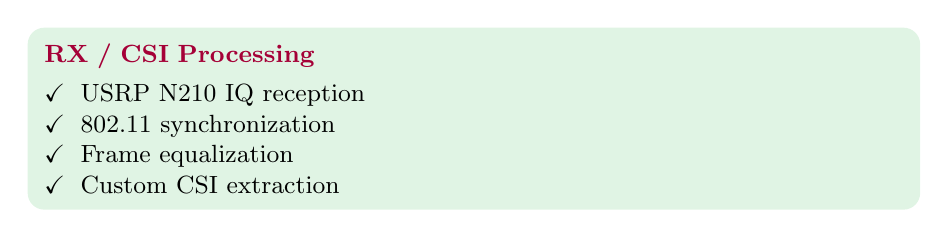
\begin{tikzpicture}
\node[
    rounded corners=6pt,
    fill=LightGreen,
    inner sep=6pt, % Reduced padding
    text width=0.9\textwidth,
    align=left,
    font=\small % Scaled down font
] {
\textbf{\color{AmritaMaroon}RX / CSI Processing}\\[3pt]
$\checkmark$\; USRP N210 IQ reception\\
$\checkmark$\; 802.11 synchronization\\
$\checkmark$\; Frame equalization\\
$\checkmark$\; Custom CSI extraction
};
\end{tikzpicture}

\end{columns}

\vspace{0.15cm} % Reduced vertical space

{\small \textbf{\color{AmritaMaroon}Current output:}
CSI measurements associated with the active channel.}

\end{center}

\end{frame}

% =========================================================
% 12. OPTIMAL SUBCARRIER SELECTION PER ACTIVITY
% =========================================================

\begin{frame}{14. Optimal Subcarrier Selection per Activity}

\vspace{0.15cm}

\begin{center}
% ---------------------------------------------------------
% IMAGE PLACEHOLDER
% ---------------------------------------------------------
\begin{tikzpicture}
\node[
    draw=AmritaMaroon,
    rounded corners=6pt,
    minimum width=0.6\paperwidth,
    minimum height=0.5\paperheight,
    align=center,
    inner sep=4pt
] {\includegraphics[width=0.6\paperwidth,height=0.5\paperheight,keepaspectratio]{optimal_sub_carrier.png}};
\end{tikzpicture}
\vspace{0.6cm}
% ---------------------------------------------------------
% CAPTION BLOCK
% ---------------------------------------------------------
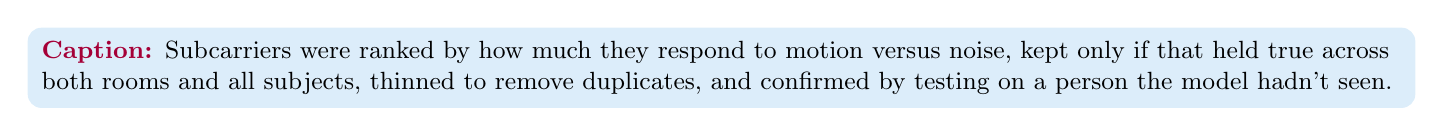
\begin{tikzpicture}
\node[
    rounded corners=5pt,
    fill=LightBlue,
    inner sep=5pt,
    text width=0.8\paperwidth,
    align=left,
    font=\small
] {
\textbf{\color{AmritaMaroon}Caption:}
Subcarriers were ranked by how much they respond to motion versus noise, kept only if that held true across both rooms and all subjects, thinned to remove duplicates, and confirmed by testing on a person the model hadn't seen.
};
\end{tikzpicture}
\vspace{0.4cm}
\end{center}
\end{frame}

% =========================================================
% 12. ACTIVE VS PASSIVE CSI SENSING
% =========================================================

\begin{frame}{13. Active vs. Passive CSI Sensing}
\subtitleline{Two paradigms for acquiring WiFi Channel State Information}

\vspace{-0.05cm}

\begin{columns}[T,totalwidth=\textwidth]

% =========================================================
% PASSIVE SENSING
% =========================================================

\column{0.48\textwidth}

\begin{center}
{\bfseries\color{AmritaMaroon} Passive Sensing}
\end{center}

\vspace{0.08cm}

\begin{center}
\begin{minipage}[c][2.7cm][c]{0.95\linewidth}
\centering
\includegraphics[width=\linewidth,height=2.7cm,keepaspectratio]{Passive.jpeg}
\end{minipage}
\end{center}

\vspace{0.12cm}

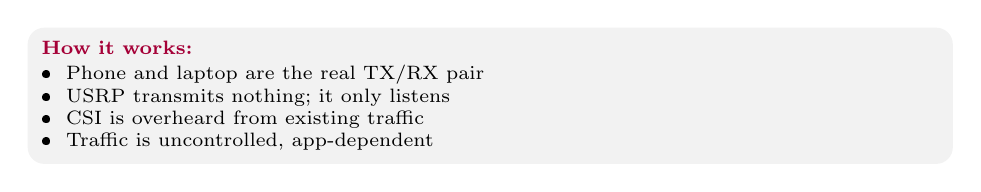
\begin{tikzpicture}
\node[
    rounded corners=6pt,
    fill=LightGray,
    inner sep=5pt,
    text width=0.94\textwidth,
    align=left,
    font=\scriptsize
] {
\textbf{\color{AmritaMaroon}How it works:}\\[1pt]
\raggedright
\textbullet\; Phone and laptop are the real TX/RX pair\\
\textbullet\; USRP transmits nothing; it only listens\\
\textbullet\; CSI is overheard from existing traffic\\
\textbullet\; Traffic is uncontrolled, app-dependent
};
\end{tikzpicture}

% =========================================================
% ACTIVE SENSING
% =========================================================

\column{0.48\textwidth}

\begin{center}
{\bfseries\color{AmritaMaroon} Active Sensing}
\end{center}

\vspace{0.08cm}

\begin{center}
\begin{minipage}[c][2.7cm][c]{0.95\linewidth}
\centering
\includegraphics[width=\linewidth,height=2.7cm,keepaspectratio]{Active.jpeg}
\end{minipage}
\end{center}

\vspace{0.12cm}

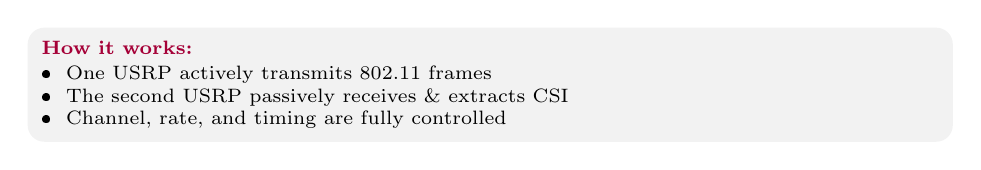
\begin{tikzpicture}
\node[
    rounded corners=6pt,
    fill=LightGray,
    inner sep=5pt,
    text width=0.94\textwidth,
    align=left,
    font=\scriptsize
] {
\textbf{\color{AmritaMaroon}How it works:}\\[1pt]
\raggedright
\textbullet\; One USRP actively transmits 802.11 frames\\
\textbullet\; The second USRP passively receives \& extracts CSI\\
\textbullet\; Channel, rate, and timing are fully controlled\\
};
\end{tikzpicture}

\end{columns}

\vspace{0.15cm}

\begin{center}
\small
\textbf{\color{AmritaMaroon}Key Insight:}
Passive sensing eavesdrops on someone else's traffic; active sensing uses a dedicated TX--RX pair for reliable, repeatable CSI.
\end{center}

\end{frame}
% =========================================================
% 13. DATA COLLECTION - WALKING & STANDING
% =========================================================

\begin{frame}{15. How the Data Was Collected: Walking \& Standing}
\subtitleline{Left: measured CSI amplitude for that take. Right: the activity being performed.}

\vspace{-0.05cm}

% ---------------- ROW 1 : WALKING ----------------
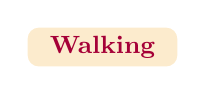
\begin{tikzpicture}
\node[rounded corners=4pt,fill=LightOrange,inner xsep=8pt,inner ysep=3pt]
{\small\bfseries\color{AmritaMaroon}Walking};
\end{tikzpicture}
{\scriptsize\color{AmritaDark}\;\;action take \textperiodcentered\ Amrith \textperiodcentered\ Room A}

\vspace{0.08cm}

\begin{columns}[c,totalwidth=\textwidth]
\column{0.62\textwidth}
\centering
\includegraphics[height=2.5cm,keepaspectratio]{ppt_images/graph_walk.png}
\column{0.36\textwidth}
\centering
\includegraphics[height=2.5cm,keepaspectratio]{ppt_images/person_walk.png}
\end{columns}

\vspace{0.22cm}

% ---------------- ROW 2 : STANDING ----------------
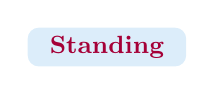
\begin{tikzpicture}
\node[rounded corners=4pt,fill=LightBlue,inner xsep=8pt,inner ysep=3pt]
{\small\bfseries\color{AmritaMaroon}Standing};
\end{tikzpicture}
{\scriptsize\color{AmritaDark}\;\;no-action take \textperiodcentered\ Rishiikesh \textperiodcentered\ Room A}

\vspace{0.08cm}

\begin{columns}[c,totalwidth=\textwidth]
\column{0.62\textwidth}
\centering
\includegraphics[height=2.5cm,keepaspectratio]{ppt_images/graph_stand.png}
\column{0.36\textwidth}
\centering
\includegraphics[height=2.5cm,keepaspectratio]{ppt_images/person_stand.png}
\end{columns}

\end{frame}


% =========================================================
% 14. DATA COLLECTION - SITTING & MIXED ACTIVITY
% =========================================================

\begin{frame}{16. How the Data Was Collected: Sitting \& Mixed Activity}
\subtitleline{Left: measured CSI amplitude for that take. Right: the activity being performed.}

\vspace{-0.05cm}

% ---------------- ROW 1 : SITTING ----------------
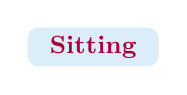
\begin{tikzpicture}
\node[rounded corners=4pt,fill=LightBlue,inner xsep=8pt,inner ysep=3pt]
{\small\bfseries\color{AmritaMaroon}Sitting};
\end{tikzpicture}
{\scriptsize\color{AmritaDark}\;\;no-action take \textperiodcentered\ Rishiikesh \textperiodcentered\ Room A}

\vspace{0.08cm}

\begin{columns}[c,totalwidth=\textwidth]
\column{0.62\textwidth}
\centering
\includegraphics[height=2.5cm,keepaspectratio]{ppt_images/graph_sit.png}
\column{0.36\textwidth}
\centering
\includegraphics[height=2.5cm,keepaspectratio]{ppt_images/person_sit.png}
\end{columns}

\vspace{0.22cm}

% ---------------- ROW 2 : MIXED ACTIVITY ----------------
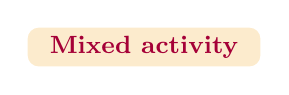
\begin{tikzpicture}
\node[rounded corners=4pt,fill=LightOrange,inner xsep=8pt,inner ysep=3pt]
{\small\bfseries\color{AmritaMaroon}Mixed activity};
\end{tikzpicture}
{\scriptsize\color{AmritaDark}\;\;action take \textperiodcentered\ Gowreesh \textperiodcentered\ Room B}

\vspace{0.08cm}

\begin{columns}[c,totalwidth=\textwidth]
\column{0.62\textwidth}
\centering
\includegraphics[height=2.5cm,keepaspectratio]{ppt_images/graph_mixed.png}
\column{0.36\textwidth}
\centering
\includegraphics[height=2.5cm,keepaspectratio]{ppt_images/person_mixed.png}
\end{columns}

\end{frame}


% =========================================================
% 17. WEARABLE FALL DETECTION   [NEW SLIDE]
% =========================================================

\begin{frame}{17. Multi-Modal Extension: Wearable Fall Detection}
\subtitleline{Edge-AI fall detection on a smartphone IMU with local IoT actuation (RO1 / RO4)}

\begin{center}
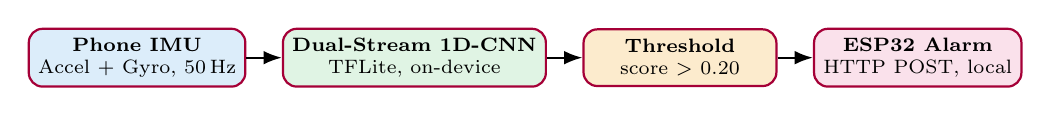
\begin{tikzpicture}[
    box/.style={
        rounded corners=5pt,
        minimum width=2.45cm,
        minimum height=0.72cm,
        align=center,
        draw=AmritaMaroon,
        thick,
        font=\scriptsize
    },
    arr/.style={-{Latex},thick}
]
\node[box,fill=LightBlue] (imu)
{\textbf{Phone IMU}\\Accel + Gyro, 50\,Hz};

\node[box,fill=LightGreen,right=0.45cm of imu] (cnn)
{\textbf{Dual-Stream 1D-CNN}\\TFLite, on-device};

\node[box,fill=LightOrange,right=0.45cm of cnn] (th)
{\textbf{Threshold}\\score $>$ 0.20};

\node[box,fill=LightPink,right=0.45cm of th] (esp)
{\textbf{ESP32 Alarm}\\HTTP POST, local};

\draw[arr] (imu)--(cnn);
\draw[arr] (cnn)--(th);
\draw[arr] (th)--(esp);
\end{tikzpicture}
\end{center}

\vspace{0.2cm}

\begin{columns}[T,totalwidth=\textwidth]

\column{0.48\textwidth}

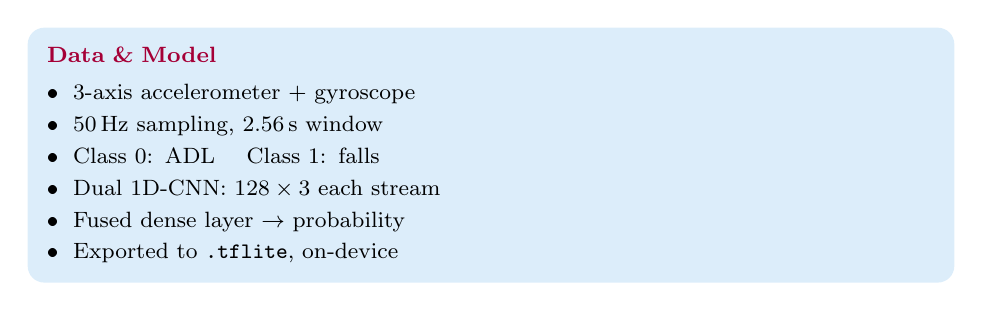
\begin{tikzpicture}
\node[
    rounded corners=6pt,
    fill=LightBlue,
    inner sep=7pt,
    text width=0.93\textwidth,
    align=left,
    font=\footnotesize
] {
\textbf{\color{AmritaMaroon}Data \& Model}\\[4pt]
\textbullet\; 3-axis accelerometer + gyroscope\\[2pt]
\textbullet\; 50\,Hz sampling, 2.56\,s window\\[2pt]
\textbullet\; Class 0: ADL \quad Class 1: falls\\[2pt]
\textbullet\; Dual 1D-CNN: $128\times3$ each stream\\[2pt]
\textbullet\; Fused dense layer $\rightarrow$ probability\\[2pt]
\textbullet\; Exported to \texttt{.tflite}, on-device
};
\end{tikzpicture}

\column{0.48\textwidth}

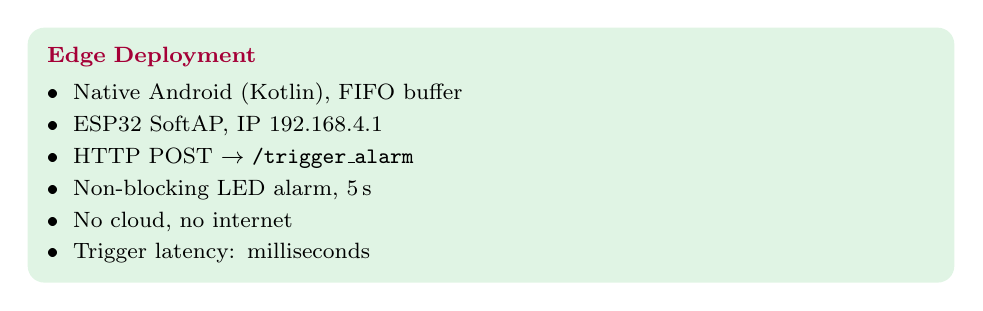
\begin{tikzpicture}
\node[
    rounded corners=6pt,
    fill=LightGreen,
    inner sep=7pt,
    text width=0.93\textwidth,
    align=left,
    font=\footnotesize
] {
\textbf{\color{AmritaMaroon}Edge Deployment}\\[4pt]
\textbullet\; Native Android (Kotlin), FIFO buffer\\[2pt]
\textbullet\; ESP32 SoftAP, IP 192.168.4.1\\[2pt]
\textbullet\; HTTP POST $\rightarrow$ \texttt{/trigger\_alarm}\\[2pt]
\textbullet\; Non-blocking LED alarm, 5\,s\\[2pt]
\textbullet\; No cloud, no internet\\[2pt]
\textbullet\; Trigger latency: milliseconds
};
\end{tikzpicture}

\end{columns}

\vspace{0.25cm}

\begin{center}
{\scriptsize
\textbf{\color{AmritaMaroon}Result:} ADL score $4.8\times10^{-4}$ vs.\ fall score $0.29$ $\rightarrow$ threshold 0.20\\[2pt]
\textbf{\color{AmritaMaroon}Open issue:} high-impact non-falls still trigger; single-user dataset
}
\end{center}

\end{frame}


% =========================================================
% 13. LIMITATIONS + FUTURE WORK
% =========================================================

\begin{frame}{18. Limitations and Future Work}
\subtitleline{What remains before full sign-language recognition}

\begin{columns}[T,totalwidth=\textwidth]

\column{0.48\textwidth}

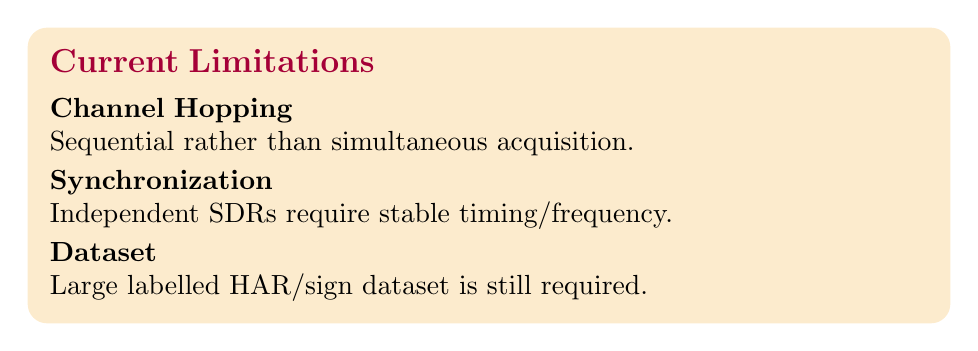
\begin{tikzpicture}
\node[
    rounded corners=7pt,
    fill=LightOrange,
    inner sep=8pt, % Reduced from 11pt
    text width=0.92\textwidth, % Increased slightly to reduce text wrapping
    align=left
] {
\textbf{\large\color{AmritaMaroon}Current Limitations}\\[4pt] % Reduced from 7pt

\textbf{Channel Hopping}\\
Sequential rather than simultaneous acquisition.\\[2pt] % Reduced from 5pt

\textbf{Synchronization}\\
Independent SDRs require stable timing/frequency.\\[2pt] % Reduced from 5pt

\textbf{Dataset}\\
Large labelled HAR/sign dataset is still required.
};
\end{tikzpicture}

\column{0.48\textwidth}

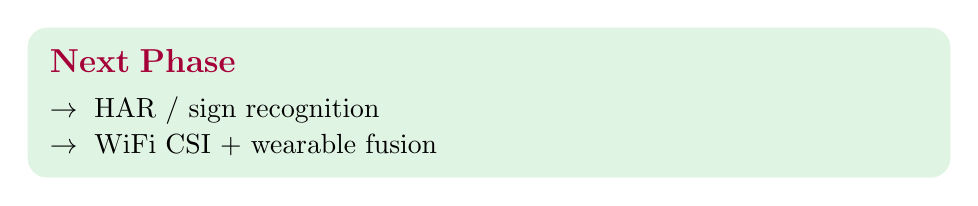
\begin{tikzpicture}
\node[
    rounded corners=7pt,
    fill=LightGreen,
    inner sep=8pt, % Reduced from 11pt
    text width=0.92\textwidth, % Increased slightly to reduce text wrapping
    align=left
] {
\textbf{\large\color{AmritaMaroon}Next Phase}\\[4pt] % Reduced from 7pt

$\rightarrow$\; HAR / sign recognition\\[1pt]
$\rightarrow$\; WiFi CSI + wearable fusion
};
\end{tikzpicture}

\end{columns}

\vspace{0.15cm} % Reduced from 0.35cm

\begin{center}
\textbf{\color{AmritaMaroon}Long-term goal:}
Sign-language recognition with identity-aware multi-modal sensing.
\end{center}

\end{frame}


% =========================================================
% 14. REFERENCES
% =========================================================

\begin{frame}{19. References}

\footnotesize % Changed from \small to prevent vertical overflow

\begin{columns}[T,totalwidth=\textwidth]

\column{0.48\textwidth}

\begin{enumerate}
\setlength{\itemsep}{3pt} % Tightened spacing between items

\item D. J. Cook et al.,
\textit{CASAS: A Smart Home in a Box},
Computer, 2013.

\item H. Alemdar et al.,
\textit{ARAS human activity datasets in multiple homes},
PervasiveHealth, 2013.

\item D. Anguita et al.,
\textit{A Public Domain Dataset for Human Activity Recognition},
ESANN, 2013.

\item R. Chavarriaga et al.,
\textit{The Opportunity challenge},
Pattern Recognition Letters, 2013.

\item D. Micucci et al.,
\textit{UniMiB SHAR},
Applied Sciences, 2017.

\item Y. Zheng et al.,
\textit{Widar3.0: Zero-Effort Cross-Domain Gesture Recognition},
IEEE TPAMI, 2021.

\end{enumerate}

\column{0.48\textwidth}

\begin{enumerate}
\setcounter{enumi}{6}
\setlength{\itemsep}{3pt} % Tightened spacing between items

\item G. Zhu et al.,
\textit{CSI-Bench},
arXiv, 2025.

\item S. Huang et al.,
\textit{WiMANS},
arXiv, 2024.

\item Y. Ma et al.,
\textit{SignFi: Sign Language Recognition Using WiFi},
ACM IMWUT, 2018.

\item J. Li et al.,
\textit{WiFinger: Finger Gesture Recognition Using CSI},
UbiComp, 2016.

\item B. D. Minor et al.,
\textit{Learning Activity Predictors from Sensor Data},
IEEE TKDE, 2017.

\vspace{0.15cm} % Reduced vertical space

\textbf{\color{AmritaMaroon}Implementation basis}\\
GNU Radio, UHD, IEEE 802.11 PHY/MAC processing,
and custom CSI extraction.

\end{enumerate}

\end{columns}

\end{frame}
% =========================================================
% THANK YOU
% =========================================================

\begin{frame}

\begin{center}

\vspace{1.2cm}

{\Huge\color{AmritaMaroon}\bfseries Thank You}

\vspace{0.5cm}

{\Large
Smart Home HAR for\\
Speech-Impaired \& Hearing-Impaired Users
}

\vspace{0.6cm}

\textbf{Guide Review 1 \;|\; Panel Review 1}

\vspace{0.4cm}

Department of Computer Science and Engineering\\
Amrita Vishwa Vidyapeetham

\end{center}

\end{frame}

\end{document}